% ═════════════════════════════════════════════════════════════════════
%  AlgoLang — An Agent-Native Programming Language for Building AI Systems
%  Presentation · Dr. S. Satyanarayana, Ph.D., PDF (AI)
%  AlgoProfessor AI R&D Solutions, Hyderabad
%
%  Build:  latexmk -xelatex algolang-slides.tex     (Overleaf: Compiler = XeLaTeX)
% ═════════════════════════════════════════════════════════════════════
\documentclass[aspectratio=169,11pt]{beamer}
\usetheme{AlgoLang}
\graphicspath{{images/}}
\newcommand{\app}[1]{../examples/apps/#1}
\newcommand{\stat}[3]{\begin{tile}{#1}{\heavy\fontsize{24}{26}\selectfont #2}\\[1mm]{\scriptsize #3}\end{tile}}
\newcommand{\ec}[3]{\begin{tcolorbox}[enhanced,colback=#1!10,colframe=#1,boxrule=0pt,leftrule=2pt,arc=1.5pt,left=3pt,right=2pt,top=1.5pt,bottom=1.5pt,before skip=0pt,after skip=2.2pt,fontupper=\scriptsize\raggedright]\textbf{\color{#1!75!black}#2}\enspace #3\end{tcolorbox}}
\newcommand{\plat}[3]{\begin{tile}{#1}{\bfseries\small #2}\\[1mm]{\ttfamily\scriptsize #3}\end{tile}}
\newcommand{\dom}[3]{\begin{tile}{#1}{\bfseries\small #2}\\[0.6mm]{\scriptsize #3}\end{tile}}
\newcommand{\pat}[3]{\begin{card}{#1}{#2}#3\end{card}}

\title{AlgoLang}
\author{Dr.\ S.\ Satyanarayana, Ph.D., PDF (AI)}
\institute{AlgoProfessor AI R\&D Solutions, Hyderabad}
\date{October 2026}
\hypersetup{pdftitle={AlgoLang — An Agent-Native Programming Language for Building AI Systems},
  pdfauthor={Dr. S. Satyanarayana, Ph.D., PDF (AI)}}

\begin{document}

% ─────────────────────────── title ───────────────────────────
\begin{frame}[plain]
\begin{tikzpicture}[remember picture,overlay]
  \fill[navy] (current page.south west) rectangle (current page.north east);
  % colour bands
  \foreach \c [count=\i] in {teal,sky,violet,rose,coral,amber,leaf,gold}
    \fill[\c] ([xshift={(\i-1)*\paperwidth/8}]current page.south west) rectangle
              ([xshift={\i*\paperwidth/8},yshift=2.2mm]current page.south west);
  \node[anchor=north east,align=left,font=\ttfamily\tiny,text=white,opacity=0.10]
    at ([xshift=-6mm,yshift=-6mm]current page.north east) {%
    agent Researcher(topic: text) -> text \{\\
    \quad goal "Find five facts about \{topic\}"\\
    \quad policy \{ require human when confidence < 0.70 \}\\
    \}\\
    flow main(topic: text) \{\\
    \quad [a, b] = par \{ Writer(t), Critic(t) \}\\
    \quad emit a, b\\
    \}};
  \node at ([xshift=-36mm,yshift=-2mm]current page.east) {\algologo[1.45]};
  \node[anchor=west,align=left] at ([xshift=12mm,yshift=10mm]current page.west) {%
    {\color{gold}\bfseries\scriptsize OPEN-SOURCE PROGRAMMING LANGUAGE · v0.1}\\[3mm]
    {\heavy\fontsize{46}{48}\selectfont\color{white}Algo\textcolor{gold}{Lang}}\\[3mm]
    {\color{white}\large An agent-native language for building AI systems}\\[1.5mm]
    {\color{white!75!navy}\normalsize Every unit of work is an \textcolor{gold}{\textbf{agent}}.}};
  \node[anchor=south west,align=left,text=white] at ([xshift=12mm,yshift=9mm]current page.south west) {%
    {\bfseries\normalsize Dr.\ S.\ Satyanarayana}\enspace{\small Ph.D., PDF (AI)}\\[0.6mm]
    {\lightf\scriptsize Founder, CEO \& Chief Agentic AI Scientist · AlgoProfessor AI R\&D Solutions, Hyderabad}\\[0.4mm]
    {\lightf\scriptsize\color{gold} www.algoprofessor.com · ceo@algoprofessor.com}};
\end{tikzpicture}
\end{frame}

% ─────────────────────────── agenda ───────────────────────────
\section{Overview}
\begin{frame}{Agenda}
\vspace{1mm}
\begin{columns}[T]
\begin{column}{0.48\textwidth}
\begin{tcolorbox}[enhanced,colback=teal,colframe=teal,arc=3pt,boxrule=0pt,left=4pt,right=4pt,top=2.5pt,bottom=2.5pt,before skip=0pt,after skip=2.6pt]
\begin{tikzpicture}[baseline=(x.base)]\node[circle,fill=white,text=teal!80!black,font=\small\bfseries,inner sep=1pt,minimum size=6mm](x){1};\end{tikzpicture}\enspace
\parbox[c]{0.8\linewidth}{\color{white}{\bfseries\small Why a new language?}\\[-0.6mm]{\scriptsize the problem and the core idea}}
\end{tcolorbox}
\begin{tcolorbox}[enhanced,colback=sky,colframe=sky,arc=3pt,boxrule=0pt,left=4pt,right=4pt,top=2.5pt,bottom=2.5pt,before skip=0pt,after skip=2.6pt]
\begin{tikzpicture}[baseline=(x.base)]\node[circle,fill=white,text=sky!80!black,font=\small\bfseries,inner sep=1pt,minimum size=6mm](x){2};\end{tikzpicture}\enspace
\parbox[c]{0.8\linewidth}{\color{white}{\bfseries\small The language}\\[-0.6mm]{\scriptsize types · agents · policies · flows}}
\end{tcolorbox}
\begin{tcolorbox}[enhanced,colback=violet,colframe=violet,arc=3pt,boxrule=0pt,left=4pt,right=4pt,top=2.5pt,bottom=2.5pt,before skip=0pt,after skip=2.6pt]
\begin{tikzpicture}[baseline=(x.base)]\node[circle,fill=white,text=violet!80!black,font=\small\bfseries,inner sep=1pt,minimum size=6mm](x){3};\end{tikzpicture}\enspace
\parbox[c]{0.8\linewidth}{\color{white}{\bfseries\small Runtime \& safety}\\[-0.6mm]{\scriptsize call lifecycle · audit log · ethics guard}}
\end{tcolorbox}
\begin{tcolorbox}[enhanced,colback=rose,colframe=rose,arc=3pt,boxrule=0pt,left=4pt,right=4pt,top=2.5pt,bottom=2.5pt,before skip=0pt,after skip=2.6pt]
\begin{tikzpicture}[baseline=(x.base)]\node[circle,fill=white,text=rose!80!black,font=\small\bfseries,inner sep=1pt,minimum size=6mm](x){4};\end{tikzpicture}\enspace
\parbox[c]{0.8\linewidth}{\color{white}{\bfseries\small Three ways to work}\\[-0.6mm]{\scriptsize command line · Studio GUI · AI writer}}
\end{tcolorbox}
\begin{tcolorbox}[enhanced,colback=coral,colframe=coral,arc=3pt,boxrule=0pt,left=4pt,right=4pt,top=2.5pt,bottom=2.5pt,before skip=0pt,after skip=2.6pt]
\begin{tikzpicture}[baseline=(x.base)]\node[circle,fill=white,text=coral!80!black,font=\small\bfseries,inner sep=1pt,minimum size=6mm](x){5};\end{tikzpicture}\enspace
\parbox[c]{0.8\linewidth}{\color{white}{\bfseries\small Inside the compiler}\\[-0.6mm]{\scriptsize pipeline · generated Python}}
\end{tcolorbox}
\end{column}
\begin{column}{0.48\textwidth}
\begin{tcolorbox}[enhanced,colback=amber,colframe=amber,arc=3pt,boxrule=0pt,left=4pt,right=4pt,top=2.5pt,bottom=2.5pt,before skip=0pt,after skip=2.6pt]
\begin{tikzpicture}[baseline=(x.base)]\node[circle,fill=white,text=amber!80!black,font=\small\bfseries,inner sep=1pt,minimum size=6mm](x){6};\end{tikzpicture}\enspace
\parbox[c]{0.8\linewidth}{\color{white}{\bfseries\small Comparison}\\[-0.6mm]{\scriptsize vs Python, Java, Rust, Mojo, Jac, Zero}}
\end{tcolorbox}
\begin{tcolorbox}[enhanced,colback=leaf,colframe=leaf,arc=3pt,boxrule=0pt,left=4pt,right=4pt,top=2.5pt,bottom=2.5pt,before skip=0pt,after skip=2.6pt]
\begin{tikzpicture}[baseline=(x.base)]\node[circle,fill=white,text=leaf!80!black,font=\small\bfseries,inner sep=1pt,minimum size=6mm](x){7};\end{tikzpicture}\enspace
\parbox[c]{0.8\linewidth}{\color{white}{\bfseries\small Real applications}\\[-0.6mm]{\scriptsize 8 domains, working code}}
\end{tcolorbox}
\begin{tcolorbox}[enhanced,colback=lilac,colframe=lilac,arc=3pt,boxrule=0pt,left=4pt,right=4pt,top=2.5pt,bottom=2.5pt,before skip=0pt,after skip=2.6pt]
\begin{tikzpicture}[baseline=(x.base)]\node[circle,fill=white,text=lilac!80!black,font=\small\bfseries,inner sep=1pt,minimum size=6mm](x){8};\end{tikzpicture}\enspace
\parbox[c]{0.8\linewidth}{\color{white}{\bfseries\small Responsible AI \& teaching}\\[-0.6mm]{\scriptsize patterns · limitations · 10 labs}}
\end{tcolorbox}
\begin{tcolorbox}[enhanced,colback=gold,colframe=gold,arc=3pt,boxrule=0pt,left=4pt,right=4pt,top=2.5pt,bottom=2.5pt,before skip=0pt,after skip=2.6pt]
\begin{tikzpicture}[baseline=(x.base)]\node[circle,fill=white,text=gold!80!black,font=\small\bfseries,inner sep=1pt,minimum size=6mm](x){9};\end{tikzpicture}\enspace
\parbox[c]{0.8\linewidth}{\color{white}{\bfseries\small Open-source project}\\[-0.6mm]{\scriptsize roadmap · licence · get started}}
\end{tcolorbox}
\end{column}
\end{columns}
\end{frame}

\begin{frame}{AlgoLang by the numbers}
\vspace{2mm}
\begin{columns}[T]
\begin{column}{0.235\textwidth}\stat{teal}{1}{primitive for work:\\ the \textbf{agent}}\stat{sky}{5}{types: text, score,\\list, json, bool}\end{column}
\begin{column}{0.235\textwidth}\stat{violet}{5}{policy rules built\\into the syntax}\stat{rose}{15}{compile-time checks\\(E100--E114)}\end{column}
\begin{column}{0.235\textwidth}\stat{coral}{3}{ways to work:\\CLI · GUI · agentic}\stat{amber}{5}{platforms: Windows, Linux,\\macOS, Docker, Colab}\end{column}
\begin{column}{0.235\textwidth}\stat{leaf}{8}{real application\\blueprints}\stat{navy2}{77}{pages of official\\documentation}\end{column}
\end{columns}
\vspace{1mm}
{\scriptsize\color{muted} Toolchain: about 3,000 lines of Python and HTML — small enough for students to read end to end.}
\end{frame}

% ═════════════════════════ 1. WHY ═════════════════════════
\partslide{teal}{01}{Why a new language?}

\begin{frame}{The problem: AI work hides inside silent functions}
\begin{columns}[T]
\begin{column}{0.47\textwidth}
In today's languages the unit of work is the \textbf{function}. When an AI model does the work inside it, nobody can easily answer:
\vspace{1mm}
\begin{enumerate}\small
  \item \textbf{Who} decided --- which worker, which model?
  \item \textbf{What} was it asked to do?
  \item With \textbf{how much confidence}?
  \item Did a \textbf{human} check it?
  \item Was a \textbf{protected attribute} (caste, gender) used?
  \item What did it \textbf{cost}, and where is the \textbf{record}?
\end{enumerate}
\end{column}
\begin{column}{0.49\textwidth}
\begin{card}{coral}{Where this matters}
Admissions · hiring · credit · healthcare · peer review · exams --- AI decisions that affect people need accountability \emph{by design}, not by afterthought.
\end{card}
\begin{card}{teal}{The AlgoLang answer}
Make each of those six questions a \textbf{part of the language}, checked by the compiler and enforced by the runtime.
\end{card}
\end{column}
\end{columns}
\end{frame}

\begin{frame}[fragile]{The core idea: agents, not functions}
\begin{columns}[T]
\begin{column}{0.44\textwidth}
\begin{tcolorbox}[enhanced,colback=navy,colframe=navy,coltext=white,arc=3pt,fontupper=\small]
{\color{gold}\bfseries The AlgoLang rule}\\[1mm]
There are \textbf{no functions}. The only thing a program can call is an \textbf{agent}. A \textbf{flow} orchestrates agents and nothing else.
\end{tcolorbox}
\vspace{1mm}
\renewcommand{\arraystretch}{1.15}
{\scriptsize
\begin{tabular}{@{}>{\bfseries\color{teal!75!black}}l l@{}}
goal & what was it asked to do?\\
role & in what capacity?\\
uses & which tools may it touch?\\
model & which model answered?\\
policy & cost, retries, human review,\\& forbidden inputs\\
audit & what happened, when?\\
\end{tabular}}
\end{column}
\begin{column}{0.53\textwidth}
\begin{algo}
agent Reviewer(draft: text) -> score {
    role   "Peer reviewer"
    goal   "Score {draft} from 0 to 1 for accuracy"
    uses   web.search
    model  smart
    policy {
        budget tokens 4000
        retry 2
        require human when confidence < 0.70
        forbid gender, caste, religion
    }
}
\end{algo}
\begin{terminal}
E101 'summarise_text' is not an agent —
     in AlgoLang every unit of work is an agent
\end{terminal}
\end{column}
\end{columns}
\end{frame}

\begin{frame}[fragile]{AlgoLang at a glance}
\begin{columns}[T]
\begin{column}{0.6\textwidth}
\begin{algo}[listing options={language=AlgoLang,basicstyle=\ttfamily\fontsize{6.5}{7.6}\selectfont}]
model fast = "claude-haiku-5-5"

agent Writer(facts: text, tone: text = "academic") -> text {
    goal  "Write a 200-word brief from {facts} in a {tone} tone"
    model fast
    policy { budget tokens 4000  retry 1 }
}

agent Reviewer(draft: text) -> score {
    goal   "Score {draft} from 0 to 1 for accuracy"
    policy { require human when confidence < 0.70 }
}

flow main(facts: text) {
    [formal, simple] = par { Writer(facts), Writer(facts, tone = "plain") }
    if Reviewer(formal) < 0.80 {
        formal = Writer(facts, tone = "rigorous academic")
    }
    emit formal, simple
}
\end{algo}
\end{column}
\begin{column}{0.37\textwidth}
\footnotesize
\begin{itemize}
  \item Two writers run \textbf{in parallel} (\kw{par})
  \item A reviewer \textbf{scores} the formal draft
  \item Low-confidence scores go to a \textbf{human}
  \item A low score triggers a \textbf{redraft}
  \item \textbf{Budgets} and \textbf{retries} on every writer
  \item Every call written to an \textbf{audit log}
  \item Everything \textbf{checked before it runs}
\end{itemize}
\end{column}
\end{columns}
\end{frame}

% ═════════════════════════ 2. LANGUAGE ═════════════════════════
\partslide{sky}{02}{The language}

\begin{frame}[fragile]{A program has four kinds of declaration}
\vspace{1mm}
\begin{columns}[T]
\begin{column}{0.24\textwidth}
\begin{card}{teal}{model}
Names a model ID; agents use the short name.
\vspace{1mm}\\\texttt{\scriptsize model smart =\\"claude-sonnet-5-5"}
\end{card}
\end{column}
\begin{column}{0.24\textwidth}
\begin{card}{violet}{tool}
Declares a capability. Gives it to \emph{no one} until an agent \kw{uses} it.
\vspace{1mm}\\\texttt{\scriptsize tool web.search}
\end{card}
\end{column}
\begin{column}{0.24\textwidth}
\begin{card}{coral}{agent}
The only unit of work: typed inputs, a return type, a goal and a policy.
\vspace{1mm}\\\texttt{\scriptsize agent A(x: text)\\-> score \{ \dots \}}
\end{card}
\end{column}
\begin{column}{0.24\textwidth}
\begin{card}{leaf}{flow}
Wires agents together. \code{flow main} is the entry point.
\vspace{1mm}\\\texttt{\scriptsize flow main(t: text)\\\{ \dots \}}
\end{card}
\end{column}
\end{columns}
\vspace{2mm}
\begin{columns}[T]
\begin{column}{0.48\textwidth}
\begin{card}{sky}{Lexical basics}
\texttt{//} comments · braces, no significant whitespace · \texttt{;} optional · strings in \texttt{"\,"} · \texttt{\{param\}} placeholders inside goals, checked by the compiler (E109)
\end{card}
\end{column}
\begin{column}{0.48\textwidth}
\begin{card}{amber}{25 keywords, no operators for computing}
Flows only \emph{route} values; all computation is done by agents. Small enough to learn in one class.
\end{card}
\end{column}
\end{columns}
\end{frame}

\begin{frame}{Five types --- and every result carries provenance}
\begin{columns}[T]
\begin{column}{0.44\textwidth}
\renewcommand{\arraystretch}{1.5}
\footnotesize
\begin{tabular}{@{}l p{45mm}@{}}
\pill{sky}{text} & free text --- facts, drafts, letters\\
\pill{coral}{score} & number 0--1; the \emph{only} comparable type\\
\pill{teal}{list} & ordered items --- the input to \kw{par for}\\
\pill{violet}{json} & structured records\\
\pill{leaf}{bool} & pass / fail checks\\
\end{tabular}
\vspace{3mm}

{\footnotesize Comparing text is a compile error:}\\[0.5mm]
\texttt{\scriptsize if summary < 0.5 \{ \dots \}\enspace\textcolor{coral}{→ E110}}
\end{column}
\begin{column}{0.52\textwidth}
\begin{tcolorbox}[enhanced,colback=navy,colframe=sky,arc=3pt,fontupper=\footnotesize\color{white},title={\bfseries Every agent call returns a Result},colbacktitle=sky,coltitle=white]
\renewcommand{\arraystretch}{1.3}
\begin{tabular}{@{}>{\ttfamily\color{gold}}l p{44mm}@{}}
value & the answer, of the declared type\\
confidence & 0--1, reported with the answer\\
agent & who produced it\\
call\_id & link to its audit record\\
status & ok · escalated · approved\\
\end{tabular}
\end{tcolorbox}
\begin{card}{amber}{Why}
Hidden uncertainty breeds over-trust; visible confidence makes it natural to route doubtful results to people.
\end{card}
\end{column}
\end{columns}
\end{frame}

\begin{frame}{Policies: governance as syntax}
\vspace{1mm}
\begin{columns}[T]
\begin{column}{0.325\textwidth}
\begin{card}{sky}{budget tokens N}
Blocks a call \emph{before} it is sent if the prompt is over budget; caps reply length in live mode.\\[0.5mm]\soft{sky}{run time}
\end{card}
\begin{card}{teal}{retry N · timeout S}
Retries failed calls; treats slow calls as failures. Policy violations are never retried.\\[0.5mm]\soft{teal}{run time}
\end{card}
\end{column}
\begin{column}{0.325\textwidth}
\begin{card}{violet}{require human when confidence < X}
Low-confidence results become \textbf{escalated}; with \code{--interactive} a person approves or rejects.\\[0.5mm]\soft{violet}{run time}
\end{card}
\begin{card}{coral}{forbid gender, caste, \dots}
Agents may not take these as inputs (E108); calls whose inputs mention them are \textbf{blocked}.\\[0.5mm]\soft{coral}{compile + run time}
\end{card}
\end{column}
\begin{column}{0.31\textwidth}
\begin{tcolorbox}[enhanced,colback=goldlight,colframe=gold,arc=3pt,boxrule=0.6pt,fontupper=\footnotesize\raggedright]
\textbf{\color{navy}Policies travel with the agent.}\\[1mm]
A caller cannot forget them, and every audit record lists the exact rules that were in force for that call.\\[2mm]
\textbf{\color{navy}No unbounded loops.}\\[1mm]
Every program finishes, and its maximum number of agent calls --- its maximum cost --- can be read from the source.
\end{tcolorbox}
\end{column}
\end{columns}
\end{frame}

\begin{frame}[fragile]{Flows: five statements, nothing else}
\begin{columns}[T]
\begin{column}{0.5\textwidth}
\renewcommand{\arraystretch}{1.45}
\scriptsize
\begin{tabular}{@{}l >{\ttfamily}l@{}}
\pill{sky}{Call} & x = Agent(a, k = v)\\
\pill{teal}{Parallel} & [a, b] = par \{ A(x), B(x) \}\\
\pill{violet}{Parallel map} & rs = par for c in xs \{ A(c) \}\\
\pill{coral}{Branch} & if s < 0.8 \{ \dots \} else \{ \dots \}\\
\pill{leaf}{Output} & emit a, b\\
\end{tabular}
\vspace{2mm}

\scriptsize
\begin{itemize}
  \item Positional or keyword arguments; defaults may be omitted
  \item Conditions compare scores, numbers, booleans
  \item Flows \textbf{cannot be called} and cannot compute
\end{itemize}
\end{column}
\begin{column}{0.47\textwidth}
\begin{algo}
flow main(paper: text) {
    criteria = Planner(paper)
    reports  = par for c in criteria {
                   CriterionReviewer(c, paper) }
    ethics   = EthicsAuditor(paper)
    verdict  = Editor(reports, ethics)
    if verdict >= 0.5 {
        letter = AcceptLetter(reports)
    } else {
        letter = RejectLetter(reports)
    }
    emit verdict, letter
}
\end{algo}
\end{column}
\end{columns}
\end{frame}

\begin{frame}{Multi-agent parallelism is a keyword}
\begin{columns}[c]
\begin{column}{0.5\textwidth}
\centering
\begin{tikzpicture}[
  ag/.style={fill=navy,text=white,rounded corners=3pt,font=\scriptsize\bfseries,minimum width=20mm,minimum height=7mm,align=center},
  pa/.style={ag,fill=sky,draw=gold,line width=1pt},
  io/.style={ellipse,fill=goldlight,draw=gold,font=\scriptsize,text=navy,minimum height=6mm},
  ar/.style={-{Stealth[length=1.8mm]},navy,line width=0.6pt}]
  \node[font=\small\bfseries,text=sky] at (0,2.15) {par \{ A, B, C \}};
  \node[io] (i) at (0,1.4) {facts};
  \node[pa] (a) at (-2.3,0.2) {Writer\\[-1pt]{\tiny formal}};
  \node[pa] (b) at (0,0.2) {Writer\\[-1pt]{\tiny plain}};
  \node[pa] (c) at (2.3,0.2) {Translator\\[-1pt]{\tiny Hindi}};
  \node[io] (o) at (0,-1.0) {[a, b, c]};
  \foreach \x in {a,b,c}{\draw[ar] (i) -- (\x); \draw[ar] (\x) -- (o);}
\end{tikzpicture}
\end{column}
\begin{column}{0.48\textwidth}
\centering
\begin{tikzpicture}[
  ag/.style={fill=navy,text=white,rounded corners=3pt,font=\scriptsize\bfseries,minimum width=19mm,minimum height=7mm,align=center},
  pa/.style={ag,fill=teal,draw=gold,line width=1pt},
  ar/.style={-{Stealth[length=1.8mm]},navy,line width=0.6pt}]
  \node[font=\small\bfseries,text=teal] at (0,2.15) {par for c in criteria \{ R(c) \}};
  \node[ag] (p) at (0,1.4) {Planner → criteria};
  \foreach \x/\l in {-2.4/novelty,-0.8/method,0.8/data,2.4/clarity}
    {\node[pa,minimum width=14mm] (r\l) at (\x,0.2) {R\\[-1pt]{\tiny \l}}; \draw[ar] (p) -- (r\l);}
  \node[ag] (s) at (0,-1.0) {Editor ← reports};
  \foreach \l in {novelty,method,data,clarity}\draw[ar] (r\l) -- (s);
\end{tikzpicture}
\end{column}
\end{columns}
\vspace{2mm}
\begin{columns}[T]
\begin{column}{0.48\textwidth}\begin{card}{sky}{Results keep their order}Names bind in the order written, whatever order agents finish.\end{card}\end{column}
\begin{column}{0.48\textwidth}\begin{card}{teal}{Fan-out / fan-in in one line}Time is roughly that of the slowest worker, not the sum.\end{card}\end{column}
\end{columns}
\end{frame}

\begin{frame}{15 compile-time checks --- before a single token is spent}
\vspace{1mm}
\begin{columns}[T]
\begin{column}{0.32\textwidth}
\ec{coral}{E101}{not an agent (the core rule)}
\ec{coral}{E102}{wrong arguments}
\ec{coral}{E103}{undefined variable}
\ec{coral}{E100}{syntax error}
\ec{coral}{E107}{defined twice}
\end{column}
\begin{column}{0.32\textwidth}
\ec{violet}{E104}{undeclared tool}
\ec{violet}{E106}{unknown model}
\ec{violet}{E108}{forbidden attribute as input}
\ec{violet}{E109}{unknown \{placeholder\} in goal}
\ec{violet}{E112}{agent without a goal}
\end{column}
\begin{column}{0.32\textwidth}
\ec{sky}{E105}{unknown type}
\ec{sky}{E110}{comparing a non-score}
\ec{sky}{E111}{no flow main}
\ec{sky}{E113}{[a, b] does not match par}
\ec{sky}{E114}{par for over a non-list}
\end{column}
\end{columns}
\vspace{1mm}
{\scriptsize \pill{coral}{correctness}\enspace\pill{violet}{governance \& capabilities}\enspace\pill{sky}{types \& structure}\qquad All errors are reported together, with line numbers. A program with errors never runs.}
\end{frame}

\begin{frame}[fragile]{The compiler at work}
\begin{columns}[T]
\begin{column}{0.4\textwidth}
\begin{algo}
agent Summariser(doc: text) -> text {
    goal "Summarise {document}"
    uses email.send
    model turbo
}
agent Screener(caste: text) -> score {
    goal "Score applicant {caste}"
    policy { forbid caste }
}
flow main(doc: text) {
    s = Summariser(doc, doc)
    t = summarise_text(doc)
    if s < 0.5 { emit s }
    emit missing
}
\end{algo}
\end{column}
\begin{column}{0.57\textwidth}
\begin{terminaltiny}
$ algo check bad_example.algo
✗ bad_example.algo: 8 error(s)
  line 5: E109 agent Summariser: goal mentions {document}
          but there is no parameter 'document'
  line 5: E104 agent Summariser uses tool 'email.send',
          which is not declared (add `tool email.send`)
  line 5: E106 agent Summariser: unknown model 'turbo'
  line 12: E108 agent Screener takes forbidden attribute
          'caste' as an input
  line 19: E102 Summariser takes 1 argument(s) (doc), got 2
  line 20: E101 'summarise_text' is not an agent — in
          AlgoLang every unit of work is an agent
  line 21: E110 's' is text, not a score
  line 22: E103 undefined variable 'missing'
\end{terminaltiny}
\end{column}
\end{columns}
\end{frame}

% ═════════════════════════ 3. RUNTIME ═════════════════════════
\partslide{violet}{03}{Runtime \& safety}

\begin{frame}{Every agent call passes through seven steps}
\vspace{3mm}
\centering
\begin{tikzpicture}[
  st/.style={fill=navy,text=white,rounded corners=3pt,font=\scriptsize,minimum width=17mm,text width=16mm,minimum height=11mm,align=center},
  ch/.style={st,fill=violet,font=\scriptsize\bfseries},
  ar/.style={-{Stealth[length=2mm]},navy,line width=0.7pt},
  stop/.style={font=\scriptsize\bfseries,text=coral,align=center}]
  \node[st] (s1) {1. bind\\arguments};
  \node[st,right=3mm of s1] (s2) {2. render\\prompt};
  \node[ch,right=3mm of s2] (s3) {3. forbid\\check};
  \node[ch,right=3mm of s3] (s4) {4. budget\\check};
  \node[st,right=3mm of s4] (s5) {5. call model\\{\tiny retry · timeout}};
  \node[ch,right=3mm of s5] (s6) {6. human\\gate};
  \node[st,fill=leaf,right=3mm of s6] (s7) {7. audit +\\return Result};
  \foreach \a/\b in {s1/s2,s2/s3,s3/s4,s4/s5,s5/s6,s6/s7} \draw[ar] (\a) -- (\b);
  \node[stop,below=3mm of $(s3.south)!0.5!(s4.south)$] {policy violation\\→ exit 2};
  \node[stop,below=3mm of s5] {fails after\\retries → exit 3};
  \node[font=\scriptsize\bfseries,text=violet,below=3mm of s6,align=center] {escalated /\\approved};
\end{tikzpicture}
\vspace{6mm}
\begin{columns}[T]
\begin{column}{0.31\textwidth}\begin{card}{violet}{Policy steps}Steps 3, 4 and 6 (purple) enforce the agent's policy on \emph{every} call.\end{card}\end{column}
\begin{column}{0.31\textwidth}\begin{card}{sky}{Concurrency}\kw{par} uses a thread pool; output and audit writes never interleave.\end{card}\end{column}
\begin{column}{0.31\textwidth}\begin{card}{leaf}{Exit codes}0 ok · 1 compile/input error · 2 policy violation · 3 agent failure\end{card}\end{column}
\end{columns}
\end{frame}

\begin{frame}[fragile]{Accountable by default: the audit log}
\begin{columns}[T]
\begin{column}{0.47\textwidth}
\begin{tcblisting}{enhanced,listing only,colback=codebg,colframe=violet,boxrule=0pt,leftrule=2.6pt,arc=2pt,left=5pt,top=2pt,bottom=2pt,
  listing options={language={},basicstyle=\ttfamily\fontsize{6.8}{8}\selectfont}}
{
  "call": "d5a1ba",
  "agent": "Researcher",
  "model": "claude-sonnet-5-5",
  "backend": "mock",
  "inputs_sha": "23cd4baf6ab210a5",
  "returns": "text",
  "confidence": 0.83,
  "tokens": 93,
  "status": "ok",
  "tools": ["web.search"],
  "policy": {"budget_tokens": 6000, "retry": 2},
  "run": "832d55bb",
  "program": "research_brief",
  "ts": "2026-10-28T11:20:13"
}
\end{tcblisting}
\end{column}
\begin{column}{0.5\textwidth}
\begin{itemize}\small
  \item \textbf{One JSON line per agent call} --- no logging code to write
  \item Records model, confidence, tokens, status, tools and the \textbf{policy in force}
  \item \textbf{Blocked} and \textbf{failed} calls recorded too, with the reason
  \item Loads straight into Excel or \code{pandas}
\end{itemize}
\begin{card}{violet}{Accountability without over-collection}
Stores a SHA-256 \emph{hash} of the prompt, not the prompt itself --- an auditor can verify an input without the log becoming a copy of sensitive data.
\end{card}
\end{column}
\end{columns}
\end{frame}

\begin{frame}[fragile]{The ethics guard in action}
\begin{columns}[T]
\begin{column}{0.38\textwidth}
\begin{algo}[listing options={language=AlgoLang,basicstyle=\ttfamily\fontsize{6.3}{7.3}\selectfont}]
agent Editor(reports: list, ethics: text)
      -> score {
  role  "Editor-in-Chief"
  goal  "Weigh {reports} and {ethics}"
  policy {
    require human when confidence < 0.75
    forbid gender, caste, religion,
           nationality
  }
}
\end{algo}
\begin{card}{coral}{What happened}
The title mentions \emph{nationality}; it reached the Editor through four reviewers, and the runtime stopped the decision.
\end{card}
\end{column}
\begin{column}{0.59\textwidth}
\begin{terminaltiny}
$ algo run paper_review.algo \
    --arg "paper=Does author nationality predict citation counts?"
▶ flow main  run=eae974c4  backend=mock
  → Planner            conf=0.71  [4 items]
  → CriterionReviewer  conf=0.70  «CriterionReviewer #1393» …
  → CriterionReviewer  conf=0.75  «CriterionReviewer #9170» …
  → CriterionReviewer  conf=0.80  «CriterionReviewer #1033» …
  → CriterionReviewer  conf=0.81  «CriterionReviewer #4612» …
  → EthicsAuditor      conf=0.79  «EthicsAuditor #1139» …
✗ POLICY VIOLATION: Editor: input mentions forbidden
  attribute 'nationality'
\end{terminaltiny}
\begin{card}{amber}{Honest limit}
The check is \emph{lexical}: it blocks the words, not proxies such as surnames or home towns. A strong safeguard, not a fairness guarantee.
\end{card}
\end{column}
\end{columns}
\end{frame}

\begin{frame}{Two backends: learn offline, deploy live}
\vspace{1mm}
\begin{columns}[T]
\begin{column}{0.48\textwidth}
\begin{tcolorbox}[enhanced,colback=leaf!8,colframe=leaf,arc=3pt,title={\bfseries Mock (default)},colbacktitle=leaf,fontupper=\small]
\begin{itemize}
  \item Free, offline, no API key
  \item \textbf{Deterministic}: same input → same output
  \item Output shaped by return type
  \item Ideal for teaching, testing, CI
\end{itemize}
\end{tcolorbox}
\end{column}
\begin{column}{0.48\textwidth}
\begin{tcolorbox}[enhanced,colback=violet!8,colframe=violet,arc=3pt,title={\bfseries Live (\texttt{--live})},colbacktitle=violet,fontupper=\small]
\begin{itemize}
  \item Real Claude models
  \item Role becomes the system persona
  \item Typed JSON reply: \texttt{\{value, confidence\}}
  \item Token budgets cap reply length
\end{itemize}
\end{tcolorbox}
\end{column}
\end{columns}
\vspace{2mm}
\centering\small
Same program, same policies, same audit log --- switch with one flag:\enspace \texttt{algo run brief.algo --arg "topic=AI" \textcolor{violet}{\textbf{--live}}}
\end{frame}

% ═════════════════════════ 4. THREE WAYS ═════════════════════════
\partslide{rose}{04}{Three ways to work}

\begin{frame}{One language, three ways to use it}
\vspace{2mm}
\begin{columns}[T]
\begin{column}{0.32\textwidth}
\begin{tcolorbox}[enhanced,colback=teal!8,colframe=teal,arc=3pt,title={\bfseries 1 · Simple: command line},colbacktitle=teal,fontupper=\footnotesize\raggedright,height=55mm]
\texttt{algo}\enspace numbered menu\\[1mm]
\texttt{algo shell}\enspace type agents line by line\\[1mm]
\texttt{algo run f.algo}\\[1mm]
\texttt{algo check f.algo}\\[2mm]
\textbf{For:} quick runs, scripts, lab sessions
\end{tcolorbox}
\end{column}
\begin{column}{0.32\textwidth}
\begin{tcolorbox}[enhanced,colback=sky!8,colframe=sky,arc=3pt,title={\bfseries 2 · Graphical},colbacktitle=sky,fontupper=\footnotesize\raggedright,height=55mm]
\texttt{algo studio}\\[1mm]
AlgoLang Studio in your browser: editor, ▶ Run, results, agent graph, Python view, problems, templates\\[2mm]
\textbf{For:} writing, running and \emph{seeing} programs
\end{tcolorbox}
\end{column}
\begin{column}{0.32\textwidth}
\begin{tcolorbox}[enhanced,colback=rose!8,colframe=rose,arc=3pt,title={\bfseries 3 · Agentic},colbacktitle=rose,fontupper=\footnotesize\raggedright,height=55mm]
\texttt{algo ask "\dots"}\\AI writes the program; the compiler checks it; errors go back for repair\\[1mm]
\texttt{algo wizard}\\six questions, no AI needed\\[2mm]
\textbf{For:} going from an idea to a program in minutes
\end{tcolorbox}
\end{column}
\end{columns}
\vspace{1mm}
\centering{\scriptsize\color{muted} All three use the same compiler and runtime: a program written one way runs unchanged in the others.}
\end{frame}

\begin{frame}[fragile]{Simple: the menu and the interactive shell}
\begin{columns}[T]
\begin{column}{0.45\textwidth}
\begin{terminaltiny}
$ algo
  AlgoLang 0.1.0 — every unit of work is an agent
   SIMPLE (command line)
     1  Create a new program    4  Interactive shell
     2  Run a program           5  Environment check
     3  Check a program for errors
   GRAPHICAL
     6  AlgoLang Studio (opens in your browser)
     7  Jupyter notebook
   AGENTIC
     8  Ask AI to write a program from your description
     9  Wizard: build a program by answering questions
     0  Exit
  Choose 0-9:
\end{terminaltiny}
\end{column}
\begin{column}{0.52\textwidth}
\begin{terminaltiny}
$ algo shell
algo> agent Explainer(topic: text) -> text {
...>     goal "Explain {topic} simply"
...> }
✓ Explainer
algo> agent Bad(x: text) -> text { goal "use {y}" }
✗ not added — 1 error(s):
  E109 line 1: goal mentions {y} but there is no parameter 'y'
algo> Explainer("graph neural networks")
  → Explainer   conf=0.64  «Explainer #8884» Explain graph…
algo> :graph
  ◇ topic        flow input
  ■ Explainer    → lesson      ← topic
  ■ QuizMaker    → quiz        ← Explainer
algo> :save lesson.algo
✓ saved lesson.algo
\end{terminaltiny}
\end{column}
\end{columns}
\end{frame}

\begin{frame}{Graphical: AlgoLang Studio}
\begin{columns}[c]
\begin{column}{0.66\textwidth}
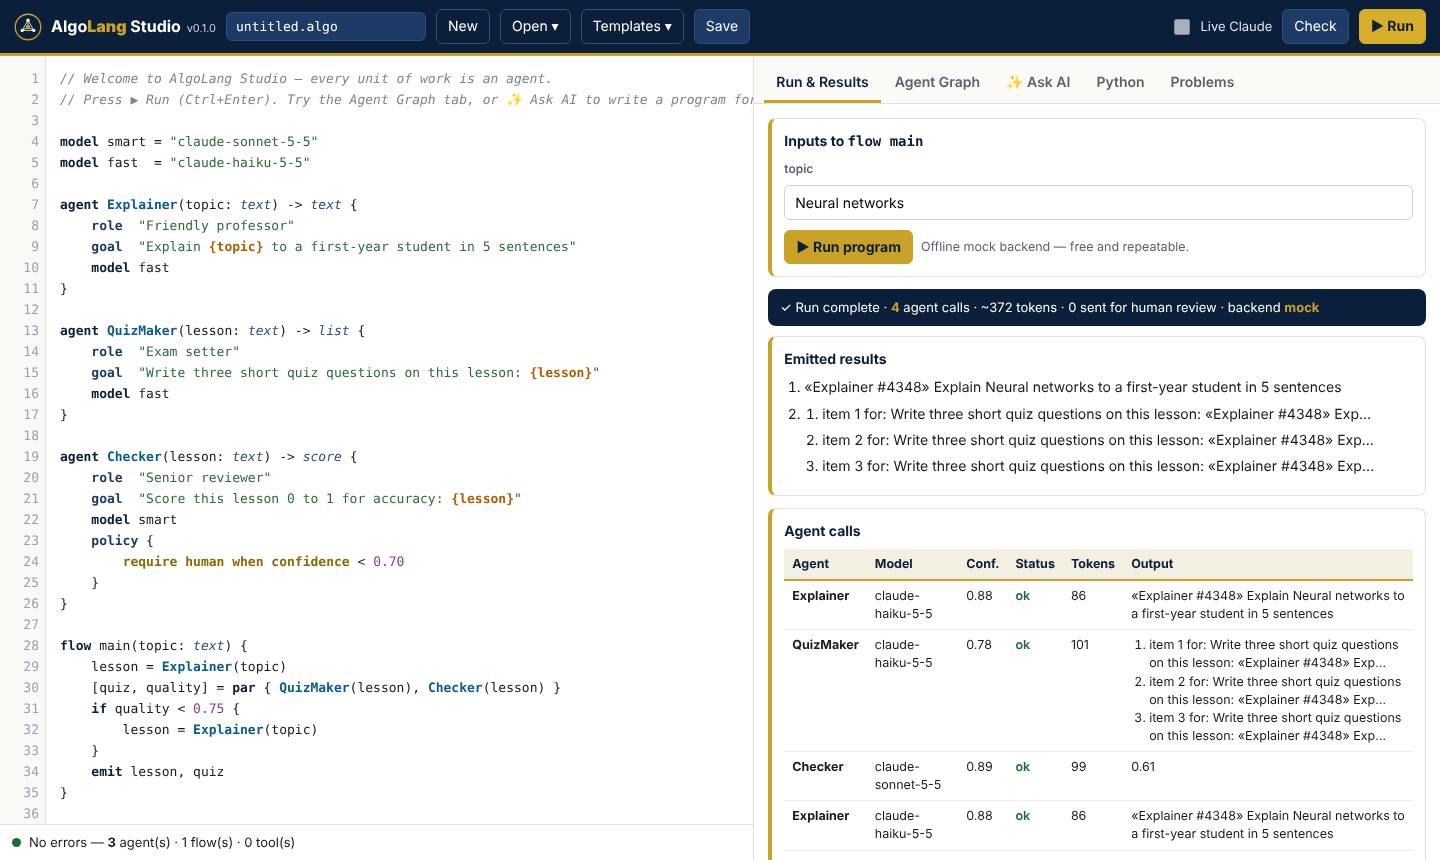
\includegraphics[width=\linewidth]{studio-run.png}
\end{column}
\begin{column}{0.32\textwidth}
\scriptsize
\begin{itemize}
  \item Highlighted editor; errors marked as you type
  \item \textbf{▶ Run} (Ctrl+Enter) with an input form
  \item Results, confidences, human-review flags
  \item Agent graph · Python · Problems
  \item Six pattern templates
  \item Local only; other sites blocked
\end{itemize}
\end{column}
\end{columns}
\end{frame}

\begin{frame}{Studio: see the agents --- and fix the errors}
\begin{columns}[T]
\begin{column}{0.255\textwidth}
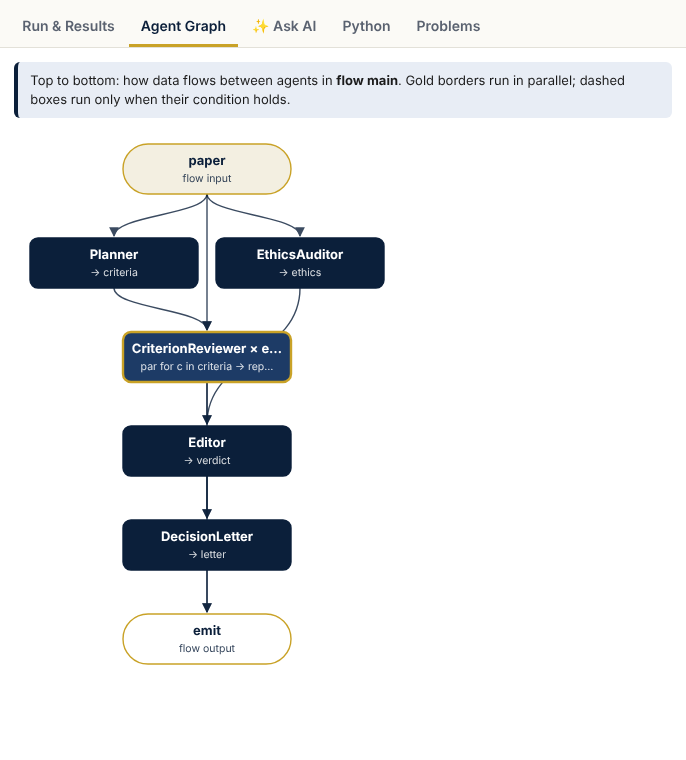
\includegraphics[width=\linewidth]{graph-paper.png}
{\tiny\centering Paper review: planner, parallel reviewers, ethics auditor, editor\par}
\end{column}
\begin{column}{0.255\textwidth}
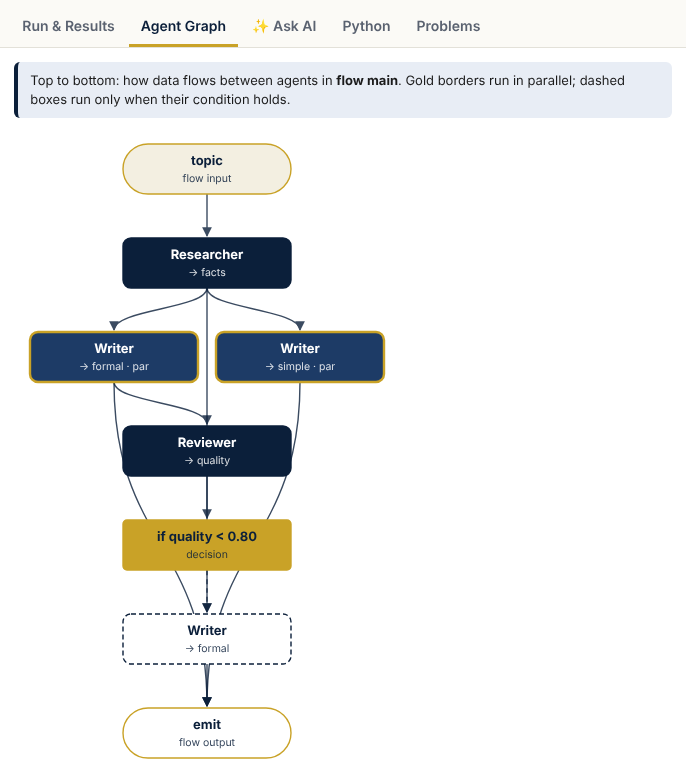
\includegraphics[width=\linewidth]{graph-brief.png}
{\tiny\centering Research brief: parallel writers, reviewer, conditional redraft\par}
\end{column}
\begin{column}{0.45\textwidth}
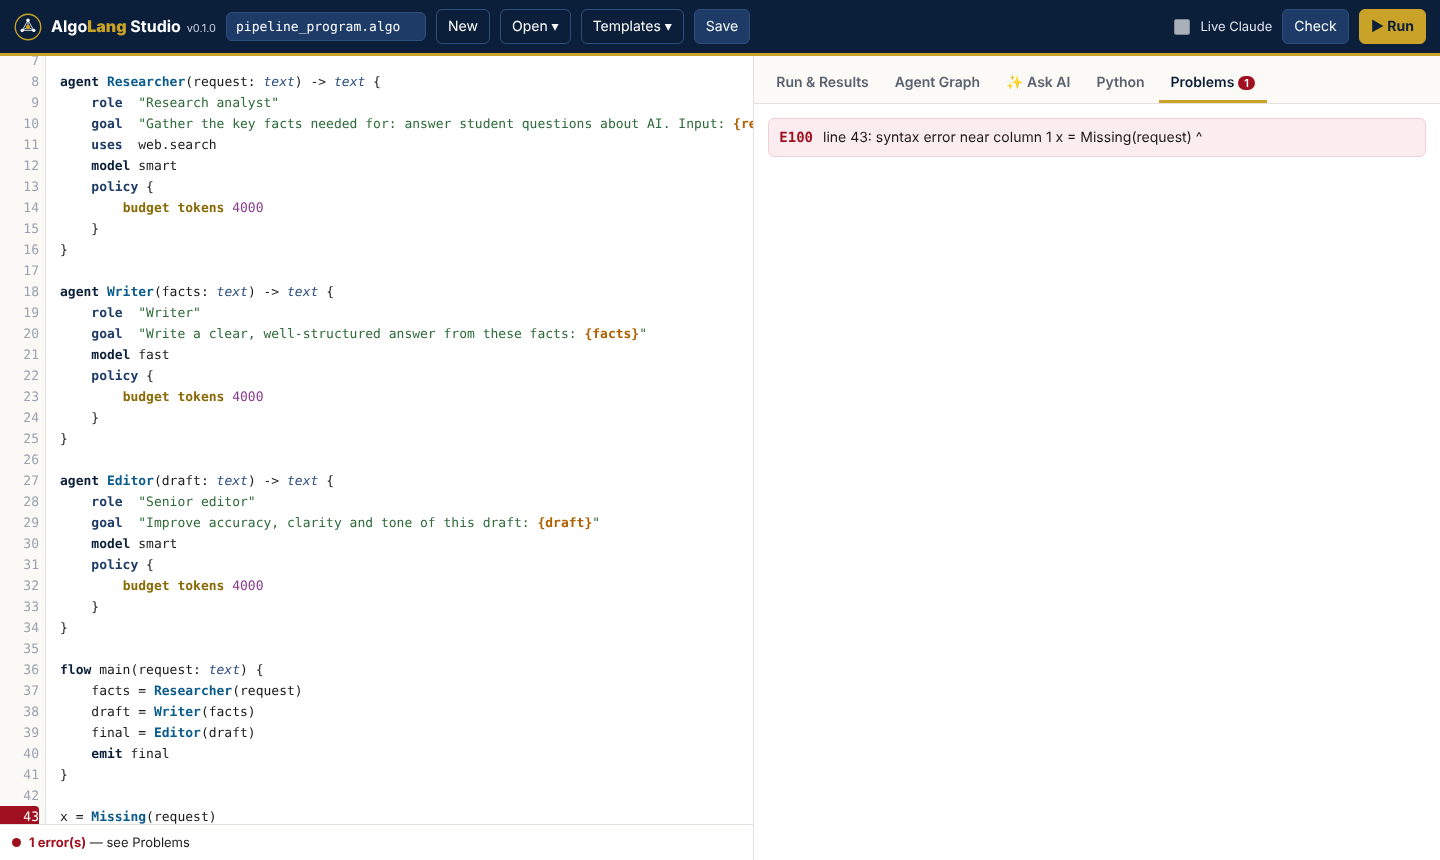
\includegraphics[width=\linewidth]{studio-problems.png}
{\tiny Problems tab: click an error to jump to its line, marked red in the margin.\par}
\vspace{2mm}
\begin{card}{sky}{Diagram legend}
\textbf{Gold border} = runs in parallel · \textbf{gold diamond} = decision · \textbf{dashed} = runs only when its condition holds
\end{card}
\end{column}
\end{columns}
\end{frame}

\begin{frame}[fragile]{Agentic: describe it --- AI writes it --- the compiler verifies it}
\begin{columns}[T]
\begin{column}{0.47\textwidth}
\centering
\begin{tikzpicture}[
  st/.style={fill=navy,text=white,rounded corners=3pt,font=\scriptsize,minimum width=19mm,minimum height=10mm,align=center},
  ar/.style={-{Stealth[length=2mm]},navy,line width=0.7pt}]
  \node[st] (r) {your\\request};
  \node[st,right=4mm of r] (m) {model writes\\AlgoLang};
  \node[st,fill=gold,text=navy,font=\scriptsize\bfseries,below=7mm of m] (c) {compiler\\checks};
  \node[st,fill=leaf,below=7mm of r] (s) {save + run\\0 errors};
  \draw[ar] (r) -- (m); \draw[ar] (m) -- (c);
  \draw[ar] (c) -- node[above,font=\tiny]{no errors} (s);
  \draw[ar,coral] (c.east) -- ++(4mm,0) |- node[pos=0.25,right,font=\tiny,text=coral,align=left]{errors\\sent back\\(max 3)} (m.east);
\end{tikzpicture}
\vspace{1mm}
\begin{terminaltiny}
$ algo ask "build a team that reviews a research paper"
\end{terminaltiny}
\begin{card}{rose}{Also in Studio}\textbf{Ask AI} tab --- with undo.\end{card}
\end{column}
\begin{column}{0.5\textwidth}
\begin{terminaltiny}
→ attempt 1: asking claude-sonnet-5-5 to write the program…
✗ attempt 1: 2 compile error(s) — sending them back
    line 2: E109 agent Reviewer: goal mentions {manuscript}
            but there is no parameter 'manuscript'
    line 7: E101 'summarise' is not an agent
→ attempt 2: asking claude-sonnet-5-5 to write the program…
✓ attempt 2: compiles with no errors
\end{terminaltiny}
\begin{card}{amber}{Still review it}
The compiler guarantees a generated program is \emph{well-formed}. Whether its goals and thresholds are \emph{right} is a human judgement.
\end{card}
\end{column}
\end{columns}
\end{frame}

\begin{frame}[fragile]{Agentic without AI: the wizard}
\begin{columns}[T]
\begin{column}{0.58\textwidth}
\begin{terminaltiny}
$ algo wizard
1. What should your AI system do: help students prepare for viva exams
2. Choose a design pattern:
   1. Pipeline        2. Fan-out / fan-in   3. Committee
   4. Critic & revise 5. Router             6. Guardrail
   Pattern number [2]: 3
3. Name of the input (one word) [request]: question
4. Send low-confidence decisions to a human? (y/n) [y]:
   Confidence threshold (0-1) [0.75]: 0.8
5. Forbid protected attributes in decisions? (y/n) [y]:
   Which ones [gender, caste, religion, nationality]:
6. Token budget per agent [4000]: 3000
✓ wrote help_students_prepare_for_viva.algo (committee
  pattern) — it compiles with no errors.
\end{terminaltiny}
\end{column}
\begin{column}{0.39\textwidth}
\begin{card}{rose}{Six questions → a working program}
Purpose · pattern · input · human review · protected attributes · budget
\end{card}
\begin{card}{leaf}{Always compiles}
Generated from tested pattern templates, with governance placed on the agent that makes the final decision.
\end{card}
\begin{card}{sky}{No API key needed}
Ideal for classrooms and first-time users.
\end{card}
\end{column}
\end{columns}
\end{frame}

\begin{frame}[fragile]{Jupyter and Google Colab}
\begin{columns}[T]
\begin{column}{0.53\textwidth}
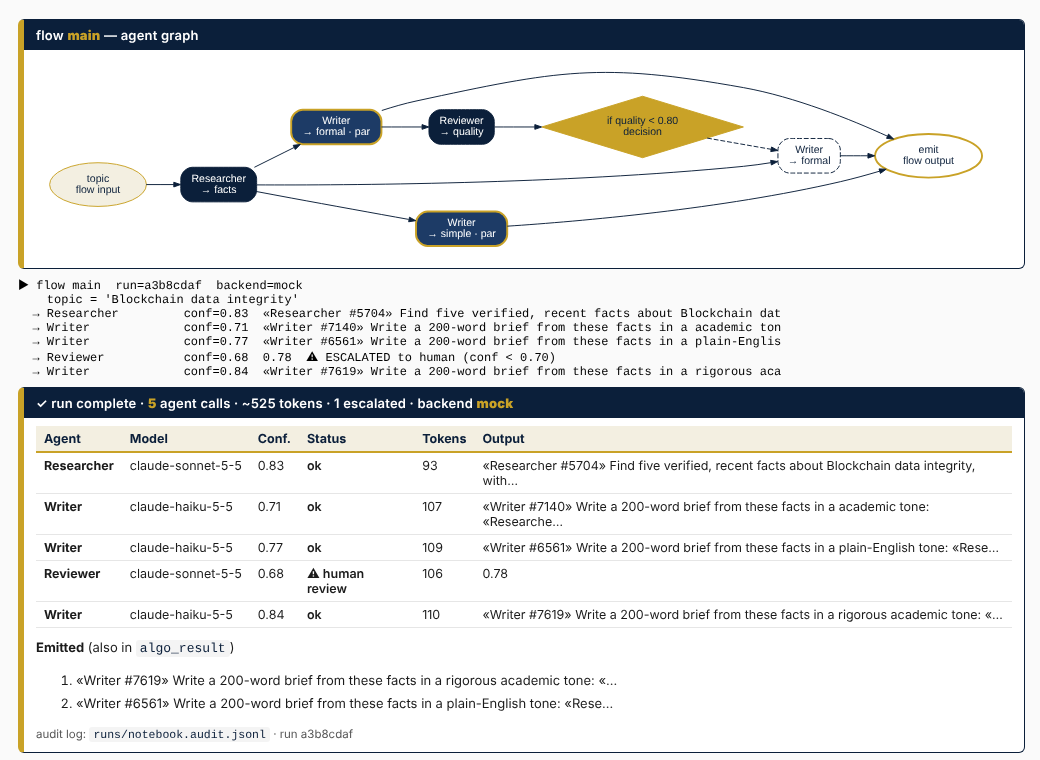
\includegraphics[width=\linewidth]{notebook.png}
\end{column}
\begin{column}{0.44\textwidth}
\begin{algo}
%%algo --arg "topic=AI ethics" --graph
flow main(topic: text) {
    facts = Researcher(topic)
    [a, b] = par { Writer(facts),
                   Critic(facts) }
    emit a, b
}
\end{algo}
\scriptsize
\begin{itemize}
  \item \textbf{Colab:} upload one notebook → \emph{Run all}
  \item \texttt{--define} cells build a program step by step
  \item \texttt{--graph} · \texttt{--check} · \texttt{--python} · \texttt{--live}
  \item Results in \texttt{algo\_result} and \texttt{algo\_calls}
\end{itemize}
\end{column}
\end{columns}
\end{frame}

\begin{frame}{Runs everywhere}
\vspace{2mm}
\begin{columns}[T]
\begin{column}{0.19\textwidth}\plat{sky}{Windows}{double-click\\install.bat}\end{column}
\begin{column}{0.19\textwidth}\plat{teal}{Linux · macOS}{bash install.sh}\end{column}
\begin{column}{0.19\textwidth}\plat{violet}{Docker}{docker run\\algolang \dots}\end{column}
\begin{column}{0.19\textwidth}\plat{amber}{Google Colab}{upload notebook\\→ Run all}\end{column}
\begin{column}{0.19\textwidth}\plat{rose}{VS Code}{syntax colours\\Ctrl+Shift+B}\end{column}
\end{columns}
\vspace{3mm}
\begin{columns}[T]
\begin{column}{0.48\textwidth}
\begin{card}{leaf}{Only one requirement}
Python 3.9+. The installer creates a private \texttt{.venv} and ends with \texttt{algo doctor}.
\end{card}
\end{column}
\begin{column}{0.48\textwidth}
\begin{card}{navy2}{Command cheat sheet}
\texttt{algo doctor · new · check · build · run · shell · studio · ask · wizard · notebook}
\end{card}
\end{column}
\end{columns}
\end{frame}

% ═════════════════════════ 5. COMPILER ═════════════════════════
\partslide{coral}{05}{Inside the compiler}

\begin{frame}[fragile]{From .algo to governed Python}
\centering
\begin{tikzpicture}[
  st/.style={fill=navy,text=white,rounded corners=3pt,font=\scriptsize,minimum width=21mm,minimum height=10mm,align=center},
  art/.style={fill=goldlight,draw=gold,text=navy,rounded corners=2pt,font=\ttfamily\scriptsize,minimum height=7mm,minimum width=12mm},
  ar/.style={-{Stealth[length=2mm]},navy,line width=0.7pt}]
  \node[art] (src) {.algo};
  \node[st,right=4mm of src] (p) {Parse\\{\tiny Lark grammar}};
  \node[st,right=4mm of p] (a) {Build AST\\{\tiny models · tools · agents}};
  \node[st,fill=coral,right=4mm of a] (c) {Check\\{\tiny 15 rules}};
  \node[st,right=4mm of c] (g) {Generate\\{\tiny Python}};
  \node[art,right=4mm of g] (py) {.py};
  \foreach \x/\y in {src/p,p/a,a/c,c/g,g/py} \draw[ar] (\x) -- (\y);
\end{tikzpicture}
\vspace{2mm}
\begin{columns}[T]
\begin{column}{0.4\textwidth}
\renewcommand{\arraystretch}{1.25}
\tiny
\begin{tabular}{@{}>{\ttfamily\color{navy}}p{24mm} >{\ttfamily}p{30mm}@{}}
\rowcolor{coral!12}\textrm{\bfseries AlgoLang} & \textrm{\bfseries Generated Python}\\
agent A(\dots) & A = rt.agent(AgentSpec(\dots))\\
A(x, k = y) & A(p1=x, k=y)\\
par \{ A(x), B(x) \} & rt.par(lambda: \dots)\\
par for v in xs \{\dots\} & rt.par\_map(lambda v: \dots)\\
if a < 0.8 & if rt.value(a) < 0.80\\
emit a, b & rt.emit(a, b)\\
\end{tabular}
\end{column}
\begin{column}{0.57\textwidth}
\begin{pycode}[listing options={style=py,basicstyle=\ttfamily\fontsize{6.4}{7.6}\selectfont}]
Researcher = rt.agent(AgentSpec(
    name='Researcher', params=[('topic', 'text', None)],
    returns='text', role='Senior research analyst',
    goal='Find five verified, recent facts about {topic}',
    uses=['web.search'], model='smart',
    policy={'budget_tokens': 6000, 'retry': 2}))

def flow_main(topic):
    facts = Researcher(topic=topic)
    formal, simple = rt.par(lambda: Writer(facts=facts),
        lambda: Writer(facts=facts, tone='plain-English'))
    quality = Reviewer(draft=formal)
    if rt.value(quality) < rt.value(0.80):
        formal = Writer(facts=facts, tone='rigorous academic')
    rt.emit(formal, simple)
\end{pycode}
\end{column}
\end{columns}
\end{frame}

% ═════════════════════════ 6. COMPARISON ═════════════════════════
\partslide{amber}{06}{Comparison with other languages}

\begin{frame}{Feature comparison: what you get out of the box}
\vspace{-1mm}
\centering
\renewcommand{\arraystretch}{1.42}
\setlength{\tabcolsep}{3.6pt}
\scriptsize
{%
\begin{tabular}{@{}l c c c c c >{\columncolor{goldlight}}c@{}}
\rowcolor{navy}\color{white}\bfseries Capability & \color{white}\bfseries Python & \color{white}\bfseries\shortstack{Python +\\agent frameworks} & \color{white}\bfseries Java / C\# & \color{white}\bfseries Rust & \color{white}\bfseries Mojo & \color{navy}\cellcolor{gold}\bfseries AlgoLang\\
Agent is a language primitive & \no & \some & \no & \no & \no & \yes\\
\rowcolor{black!3}Compile-time check of agent wiring & \no & \no & \some & \some & \some & \yes\\
Enforced per-agent tool capabilities & \no & \some & \no & \no & \no & \yes\\
\rowcolor{black!3}Human review on low confidence & \no & \some & \no & \no & \no & \yes\\
Protected-attribute guard & \no & \no & \no & \no & \no & \yes\\
\rowcolor{black!3}Per-agent token budget & \no & \some & \no & \no & \no & \yes\\
Automatic per-call audit trail & \no & \some & \no & \no & \no & \yes\\
\rowcolor{black!3}Parallel agents as a keyword & \some & \some & \some & \some & \some & \yes\\
AI writer with compiler-verified repair & \no & \no & \no & \no & \no & \yes\\
\rowcolor{black!3}Mature library ecosystem & \yes & \yes & \yes & \yes & \some & \no\\
Raw performance & \some & \some & \yes & \yes & \yes & \some\\
\rowcolor{black!3}General-purpose computing & \yes & \yes & \yes & \yes & \yes & \no\\
\end{tabular}}
\vspace{1.5mm}

{\tiny \yes\ built in\quad \some\ possible via libraries, add-ons or hand-written code\quad \no\ not available\qquad Author's assessment of built-in support, October 2026. ``Agent frameworks'' = e.g.\ LangGraph, CrewAI.}
\end{frame}

\begin{frame}{Where AlgoLang wins --- and where others win}
\vspace{1mm}
\begin{columns}[T]
\begin{column}{0.48\textwidth}
\begin{tcolorbox}[enhanced,colback=leaf!7,colframe=leaf,arc=3pt,title={\bfseries AlgoLang is stronger at},colbacktitle=leaf,fontupper=\scriptsize\raggedright]
\begin{itemize}
  \item Making AI work \textbf{visible}: every worker is declared
  \item Catching wiring mistakes \textbf{before} any API spend
  \item Governance that cannot be \textbf{forgotten} by a caller
  \item \textbf{Bounded} programs: maximum cost readable from source
  \item \textbf{Teaching} agentic AI and AI ethics with real code
\end{itemize}
\end{tcolorbox}
\end{column}
\begin{column}{0.48\textwidth}
\begin{tcolorbox}[enhanced,colback=amber!8,colframe=amber,arc=3pt,title={\bfseries Others are stronger at},colbacktitle=amber,fontupper=\scriptsize\raggedright]
\begin{itemize}
  \item \textbf{Ecosystem}: Python's libraries, community, tooling
  \item \textbf{Performance}: Rust, C++, Mojo for compute-heavy work
  \item \textbf{General computing}: AlgoLang deliberately has no arithmetic or loops
  \item \textbf{Maturity}: v0.1 is a preview; tools are declared but not yet executed
\end{itemize}
\end{tcolorbox}
\end{column}
\end{columns}
\vspace{1mm}
\begin{tcolorbox}[enhanced,colback=navy,colframe=navy,coltext=white,arc=3pt,fontupper=\small,halign=center]
\hyphenpenalty=10000 AlgoLang is not a replacement for Python.\\ It is the \textcolor{gold}{\textbf{governed orchestration layer}} --- and it compiles \emph{to} Python.
\end{tcolorbox}
\end{frame}

\begin{frame}[fragile]{Same program, two languages}
\begin{columns}[T]
\begin{column}{0.53\textwidth}
{\scriptsize\bfseries\color{muted} Plain Python — governance written by hand (excerpt of 36 lines)}
\begin{pycode}[listing options={style=py,basicstyle=\ttfamily\fontsize{5.6}{6.6}\selectfont}]
def agent(name, role, goal, model, budget=None,
          human_below=None, forbid=(), **args):
    prompt = f"ROLE: {role}\nGOAL: " + goal.format(**args)
    for word in forbid:
        if re.search(rf"\b{word}\b", prompt, re.I):
            raise PermissionError(f"{name}: forbidden {word}")
    if budget and len(prompt) // 4 > budget:
        raise PermissionError(f"{name}: over token budget")
    out = call_llm(model, role, prompt, budget or 2000)
    status = ("escalated" if human_below and
              out["confidence"] < human_below else "ok")
    AUDIT.write(json.dumps({"agent": name, "status": status,
        "confidence": out["confidence"], "ts": time.time()}))
    return out["value"], out["confidence"]

def main(topic):
    facts, _ = agent("Researcher", "Senior research analyst",
        "Find five verified facts about {topic}",
        "claude-sonnet-5-5", budget=6000, topic=topic)
    with ThreadPoolExecutor() as pool:
        f1 = pool.submit(agent, "Writer", ..., facts=facts)
        ...
\end{pycode}
\end{column}
\begin{column}{0.44\textwidth}
\begin{card}{amber}{Similar length --- different guarantees}
Both versions are about 37 lines. The difference is \emph{what is guaranteed}:
\end{card}
\vspace{-1mm}
\renewcommand{\arraystretch}{1.2}
\tiny
\begin{tabular}{@{}p{26mm} p{14mm} p{14mm}@{}}
\rowcolor{navy}\color{white}\bfseries Mistake & \color{white}\bfseries Python & \color{white}\bfseries AlgoLang\\
Typo in \texttt{\{facts\}} & crash at run time & E109 before running\\
\rowcolor{black!3}Call a missing agent & crash at run time & E101 before running\\
Forgot \texttt{forbid} on one call & silently unguarded & policy is on the agent\\
\rowcolor{black!3}Forgot audit on one call & silently missing & always written\\
Unbounded retry loop & possible & impossible\\
\end{tabular}
\vspace{1mm}

{\tiny\color{muted} Both programs were run; the Python version used a stub model.}
\end{column}
\end{columns}
\end{frame}

\begin{frame}{The new wave of agent-era languages}
\vspace{1mm}
\begin{columns}[T]
\begin{column}{0.48\textwidth}
\begin{card}{sky}{Jac / Jaseci --- University of Michigan}
Python-like language and runtime that treat AI and AI agents as first-class entities.
\end{card}
\begin{card}{violet}{Zero --- Vercel Labs (May 2026)}
Experimental systems language designed for AI \emph{coding} agents: structured compiler output, explicit effects, predictable memory.
\end{card}
\end{column}
\begin{column}{0.48\textwidth}
\begin{card}{teal}{nanolang --- Jordan Hubbard (2026)}
Minimal, LLM-friendly language with mandatory testing and unambiguous syntax.
\end{card}
\begin{card}{coral}{Mojo --- Modular}
Python-family language focused on high performance for AI and ML code.
\end{card}
\end{column}
\end{columns}
\begin{tcolorbox}[enhanced,colback=goldlight,colframe=gold,boxrule=0.6pt,arc=3pt,fontupper=\footnotesize,before skip=1mm,after skip=1mm]
\textbf{\color{navy}AlgoLang's distinct focus:} \textbf{governance of multi-agent systems} --- human oversight, protected attributes, budgets, capabilities and audit built into the syntax, plus a teaching-first toolchain.
\end{tcolorbox}
{\tiny\color{muted} Sources: The Register (Oct 2026) on Jac; Vercel Labs / noqta.tn (May 2026) on Zero; Simon Willison (Jan 2026) on nanolang.}
\end{frame}

% ═════════════════════════ 7. APPLICATIONS ═════════════════════════
\partslide{leaf}{07}{Real applications}

\begin{frame}{Eight domains, eight working programs}
\vspace{1mm}
\begin{columns}[T]
\begin{column}{0.24\textwidth}\dom{sky}{Education}{AI tutor, quiz,\\graded with oversight}\dom{coral}{Healthcare}{clinical-note triage\\with a human gate}\end{column}
\begin{column}{0.24\textwidth}\dom{violet}{Finance \& scholarships}{fair screening,\\separate auditor}\dom{rose}{Cybersecurity}{parallel log triage,\\incident report}\end{column}
\begin{column}{0.24\textwidth}\dom{teal}{Customer support}{route each ticket\\to a specialist}\dom{navy2}{Legal}{contract clause\\risk review}\end{column}
\begin{column}{0.24\textwidth}\dom{leaf}{Agriculture}{crop advice in\\Hindi, Marathi, Telugu}\dom{amber}{Research}{literature review\\for Ph.D.\ scholars}\end{column}
\end{columns}
\vspace{2mm}
\centering{\scriptsize\color{muted} Every program on the next slides is printed from its real file in \texttt{examples/apps/}, and every one compiles and runs.}
\end{frame}

% application slides — code printed from examples/apps/*.algo
\partcolor{sky}
\begin{frame}{Education: an AI tutor that explains, quizzes and grades}
\begin{columns}[T]
\begin{column}{0.63\textwidth}\algofile{\app{edu_tutor.algo}}\end{column}
\begin{column}{0.35\textwidth}
\centering\chain{Tutor,{QuizMaker\,\,\textbar\,\,Grader (par)},Tutor (redraft if weak)}\par\vspace{2mm}
\raggedright{\pill{sky}{par}\ \pill{violet}{human review}\ \pill{amber}{redraft}}\par\vspace{1.5mm}
\begin{card}{sky}{Impact}Personalised lessons for every level; a grader's uncertain marks go to the teacher, not the student.\end{card}
\end{column}
\end{columns}
\end{frame}

\partcolor{coral}
\begin{frame}{Healthcare: clinical-note triage with a human gate}
\begin{columns}[T]
\begin{column}{0.63\textwidth}\algofile{\app{health_triage.algo}}\end{column}
\begin{column}{0.35\textwidth}
\centering\chain{Summariser,RiskScorer,{Referral (if urgent)}}\par\vspace{2mm}
\raggedright{\pill{violet}{human < 0.95}\ \pill{coral}{forbid}\ \pill{sky}{branch}}\par\vspace{1.5mm}
\begin{card}{coral}{Impact}Faster triage, with a very high review threshold: the doctor decides. Decision support, never diagnosis.\end{card}
\end{column}
\end{columns}
\end{frame}

\partcolor{violet}
\begin{frame}{Finance \& scholarships: fair screening}
\begin{columns}[T]
\begin{column}{0.63\textwidth}\algofile{\app{fair_screening.algo}}\end{column}
\begin{column}{0.35\textwidth}
\centering\chain{Splitter,{Scorer × each (par for)},FairnessAuditor}\par\vspace{2mm}
\raggedright{\pill{coral}{forbid 4 attributes}\ \pill{violet}{human}\ \pill{sky}{budget}}\par\vspace{1.5mm}
\begin{card}{violet}{Impact}Merit-only scoring; an \emph{independent} auditor checks outcomes across groups --- separation of duties.\end{card}
\end{column}
\end{columns}
\end{frame}

\partcolor{rose}
\begin{frame}{Cybersecurity: parallel log triage}
\begin{columns}[T]
\begin{column}{0.63\textwidth}\algofile{\app{cyber_logs.algo}}\end{column}
\begin{column}{0.35\textwidth}
\centering\chain{Splitter,{Detector × each window},Severity,Report}\par\vspace{2mm}
\raggedright{\pill{teal}{par for}\ \pill{sky}{budget + retry}\ \pill{violet}{human}}\par\vspace{1.5mm}
\begin{card}{rose}{Impact}Many log windows analysed at once; a SOC analyst reviews uncertain severity before escalation.\end{card}
\end{column}
\end{columns}
\end{frame}

\partcolor{teal}
\begin{frame}{Customer support: route every ticket}
\begin{columns}[T]
\begin{column}{0.63\textwidth}\algofile{\app{support_router.algo}}\end{column}
\begin{column}{0.35\textwidth}
\centering\chain{IsTechnical,{TechSupport \textbar\ Billing},ToneCheck}\par\vspace{2mm}
\raggedright{\pill{sky}{router}\ \pill{amber}{quality gate}}\par\vspace{1.5mm}
\begin{card}{teal}{Impact}Each ticket reaches the right specialist; replies are checked for tone before they go out.\end{card}
\end{column}
\end{columns}
\end{frame}

\partcolor{navy2}
\begin{frame}{Legal: contract clause risk review}
\begin{columns}[T]
\begin{column}{0.63\textwidth}\algofile{\app{legal_contract.algo}}\end{column}
\begin{column}{0.35\textwidth}
\centering\chain{ClauseFinder,{ClauseRisk × each clause},RiskScore}\par\vspace{2mm}
\raggedright{\pill{teal}{par for}\ \pill{violet}{human < 0.90}\ \pill{sky}{file.read}}\par\vspace{1.5mm}
\begin{card}{navy2}{Impact}Every clause reviewed in parallel; the lawyer signs off whenever the model is not highly confident.\end{card}
\end{column}
\end{columns}
\end{frame}

\partcolor{leaf}
\begin{frame}{Agriculture: crop advice in three Indian languages}
\begin{columns}[T]
\begin{column}{0.63\textwidth}\algofile{\app{agri_advisory.algo}}\end{column}
\begin{column}{0.35\textwidth}
\centering\chain{Advisor,SafetyCheck,{Hindi \textbar\ Marathi \textbar\ Telugu}}\par\vspace{2mm}
\raggedright{\pill{coral}{guardrail}\ \pill{teal}{par translate}\ \pill{sky}{web.search}}\par\vspace{1.5mm}
\begin{card}{leaf}{Impact}Weather-aware advice reaches farmers in their own language --- only after a pesticide-safety check.\end{card}
\end{column}
\end{columns}
\end{frame}

\partcolor{amber}
\begin{frame}{Research: literature review for Ph.D.\ scholars}
\begin{columns}[T]
\begin{column}{0.63\textwidth}\algofile{\app{lit_review.algo}}\end{column}
\begin{column}{0.35\textwidth}
\centering\chain{Searcher,{Reader × each paper},GapFinder,Writer}\par\vspace{2mm}
\raggedright{\pill{teal}{fan-out / fan-in}\ \pill{sky}{web.search}}\par\vspace{1.5mm}
\begin{card}{amber}{Impact}Six papers read in parallel, gaps identified, a related-work draft produced --- for the scholar to verify.\end{card}
\end{column}
\end{columns}
\end{frame}
\partcolor{leaf}

\begin{frame}{Also built in: academic peer review}
\begin{columns}[c]
\begin{column}{0.36\textwidth}
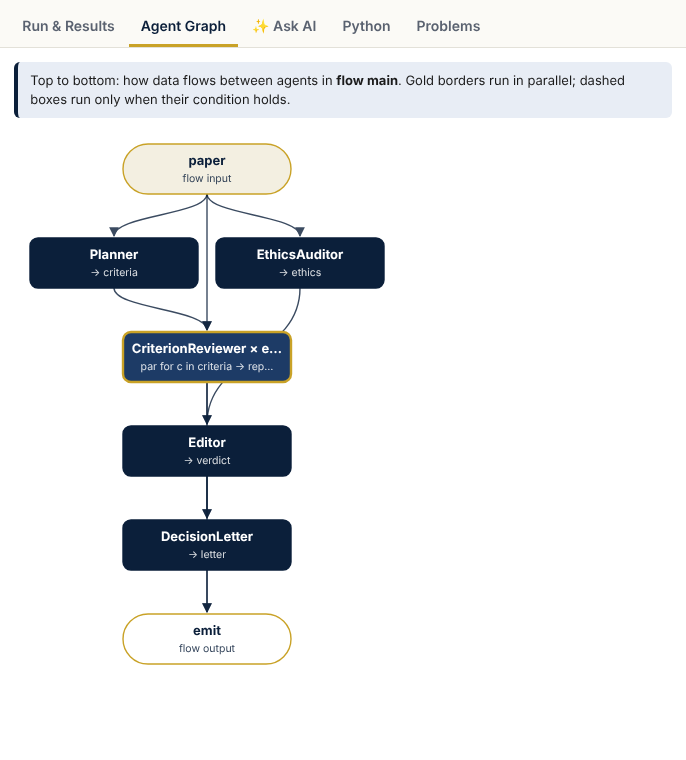
\includegraphics[width=0.9\linewidth]{graph-paper.png}
\end{column}
\begin{column}{0.6\textwidth}
\begin{card}{leaf}{paper\_review.algo --- an editorial office in 50 lines}
\begin{enumerate}\footnotesize
  \item \textbf{Planner} picks the review criteria
  \item \textbf{CriterionReviewer} runs once per criterion, in parallel
  \item \textbf{EthicsAuditor} checks consent, bias, reproducibility
  \item \textbf{Editor} scores --- blind to author identity (\texttt{forbid})
  \item \textbf{DecisionLetter} drafts a courteous letter
\end{enumerate}
\end{card}
\begin{card}{amber}{Who it is for}
Journal editors, conference chairs and Ph.D.\ supervisors who want faster, fairer, auditable first-round reviews.
\end{card}
\end{column}
\end{columns}
\end{frame}

% ═════════════════════════ 8. RESPONSIBLE AI ═════════════════════════
\partslide{lilac}{08}{Responsible AI \& teaching}

\begin{frame}{Eight multi-agent design patterns}
\vspace{1mm}
\begin{columns}[T]
\begin{column}{0.24\textwidth}\pat{sky}{Pipeline}{Stages with different skills}\pat{teal}{Fan-out / fan-in}{Speed on decomposable work}\end{column}
\begin{column}{0.24\textwidth}\pat{violet}{Committee}{Several experts, one judge}\pat{coral}{Critic \& revise}{Bounded rounds of improvement}\end{column}
\begin{column}{0.24\textwidth}\pat{amber}{Router}{Right specialist per input}\pat{rose}{Guardrail}{Safety check before work}\end{column}
\begin{column}{0.24\textwidth}\pat{leaf}{Human-in-the-loop}{Gate the decisions that matter}\pat{navy2}{Separation of duties}{Decider $\neq$ auditor}\end{column}
\end{columns}
\vspace{1mm}
\centering{\scriptsize\color{muted} The first six are available as one-click templates in Studio and in \texttt{algo wizard}.}
\end{frame}

\begin{frame}{Responsible AI: principles mapped to features}
\vspace{-1mm}
\centering
\renewcommand{\arraystretch}{1.3}
\scriptsize
\begin{tabular}{@{}>{\bfseries\color{navy}}m{28mm} >{\raggedright\arraybackslash}m{72mm} >{\ttfamily\color{navy2}\raggedright\arraybackslash}m{30mm}@{}}
\rowcolor{navy}\color{white}Principle & \color{white}\bfseries How AlgoLang supports it & \color{white}\bfseries\rmfamily Feature\\
Accountability & Every unit of work is named and has a goal; every call recorded & agents only, audit log\\
\rowcolor{black!3}Human oversight & Low-confidence results routed to people; reviewers approve & require human when\\
Fairness & Protected attributes rejected as inputs and blocked in prompts & forbid (E108)\\
\rowcolor{black!3}Transparency & Capabilities, models, policies visible in source and logs & tool, uses, model\\
Security & Agents receive only explicitly granted capabilities & declared tools (E104)\\
\rowcolor{black!3}Privacy & Log stores prompt hashes, not prompts or outputs & inputs\_sha\\
Sustainability \& cost & Per-agent budgets; no unbounded loops & budget tokens\\
\rowcolor{black!3}Reliability & Retries, timeouts, deterministic offline testing & retry, timeout, mock\\
\end{tabular}
\vspace{1mm}

{\tiny\color{muted} Produces evidence useful for frameworks such as the NIST AI RMF and the EU AI Act's record-keeping and human-oversight provisions --- but no language alone makes a system compliant.}
\end{frame}

\begin{frame}{Known limitations of version 0.1}
\vspace{1mm}
\begin{columns}[T]
\begin{column}{0.48\textwidth}
\begin{card}{coral}{forbid is lexical}Blocks the words, not proxies (surname, town, school).\end{card}
\begin{card}{amber}{Confidence is self-reported}Not a calibrated probability; validate before trusting thresholds.\end{card}
\begin{card}{violet}{Tools are declared, not executed}Executable tool bindings (incl.\ MCP) planned for v0.3.\end{card}
\end{column}
\begin{column}{0.48\textwidth}
\begin{card}{sky}{Argument types not yet checked}Planned for v0.2; flow inputs arrive as text.\end{card}
\begin{card}{teal}{Prompt injection}Policies limit what agents can do, but do not detect injected instructions.\end{card}
\begin{card}{rose}{Audit log is a local file}Not tamper-proof --- protect and back it up.\end{card}
\end{column}
\end{columns}
\vspace{0.5mm}
\centering{\scriptsize\bfseries\color{coral} Not for sole use in legally significant decisions about people without independent validation and human review.}
\end{frame}

\begin{frame}{Teaching with AlgoLang: a 10-lab module}
\vspace{-1mm}
\centering
\renewcommand{\arraystretch}{1.22}
\scriptsize
\begin{tabular}{@{}>{\bfseries\color{lilac!80!black}}c m{30mm} m{68mm} m{28mm}@{}}
\rowcolor{navy}\color{white}\bfseries Lab & \color{white}\bfseries Topic & \color{white}\bfseries Students build & \color{white}\bfseries Concepts\\
1 & First agents & The starter program; change goals and roles & agent, goal, flow\\
\rowcolor{black!3}2 & Types and scores & A grader that returns a score, and a branch & types, if, E110\\
3 & Reading errors & Fix a program with eight errors & diagnostics\\
\rowcolor{black!3}4 & Parallel agents & A committee of three experts and a judge & par\\
5 & Planning & A planner and par for workers & fan-out / fan-in\\
\rowcolor{black!3}6 & Capabilities & Grant and remove tools & least privilege\\
7 & Human oversight & Gate a decision agent; --interactive & thresholds\\
\rowcolor{black!3}8 & Fairness & Screening with forbid; probe with proxies & fairness limits\\
9 & Audit & Load the audit log into pandas & accountability\\
\rowcolor{black!3}10 & Going live & Run a finished flow on Claude with budgets & cost, real output\\
\end{tabular}
\vspace{1mm}

{\scriptsize\color{muted} Free and repeatable on the mock backend; zero installation in Google Colab.}
\end{frame}

% ═════════════════════════ 9. PROJECT ═════════════════════════
\partslide{gold}{09}{The open-source project}

\begin{frame}{Roadmap}
\vspace{4mm}
\centering
\begin{tikzpicture}[
  ms/.style={circle,draw=white,line width=1.2pt,minimum size=6mm,inner sep=0pt},
  lab/.style={font=\bfseries\small,text=navy,anchor=south},
  txt/.style={font=\scriptsize,text=ink,align=left,anchor=north,text width=33mm}]
  \fill[navylight] (-0.4,-0.18) rectangle (13.6,0.18);
  \fill[gold] (-0.4,-0.18) rectangle (1.2,0.18);
  \node[ms,fill=gold] at (1.2,0) {}; \node[lab] at (1.2,0.42) {v0.1 · now};
  \node[ms,fill=sky] at (5.0,0) {}; \node[lab] at (5.0,0.42) {v0.2};
  \node[ms,fill=violet] at (8.8,0) {}; \node[lab] at (8.8,0.42) {v0.3};
  \node[ms,fill=leaf] at (12.6,0) {}; \node[lab] at (12.6,0.42) {v1.0};
  \node[txt] at (1.7,-0.45) {Agents, flows, policies\\par / par for\\mock + live backends\\audit log · notebooks\\Studio · shell · ask · wizard};
  \node[txt] at (5.0,-0.45) {Argument type checking\\\texttt{uncertain<T>} type\\\texttt{eval} blocks with\\trace replay\\language server};
  \node[txt] at (8.8,-0.45) {Executable tools\\(MCP bindings)\\cost \& energy budgets\\consent-scoped memory};
  \node[txt] at (12.6,-0.45) {Stable language\\typed agent messaging\\native runtime\\package registry};
\end{tikzpicture}
\vspace{4mm}
\begin{columns}[T]
\begin{column}{0.48\textwidth}\begin{card}{gold}{Semantic versioning}From 1.0, programs that compile under 1.$x$ compile under every later 1.$y$.\end{card}\end{column}
\begin{column}{0.48\textwidth}\begin{card}{violet}{AlgoLang Enhancement Proposals}Every proposal must include a section on its responsible-AI implications.\end{card}\end{column}
\end{columns}
\end{frame}

\begin{frame}[fragile]{Open source: licence, contributions, citation}
\vspace{1mm}
\begin{columns}[T]
\begin{column}{0.44\textwidth}
\begin{card}{leaf}{Licence}
Software: \textbf{Apache 2.0}\enspace·\enspace Documentation: \textbf{CC BY 4.0}
\end{card}
\begin{card}{sky}{Contribute}
Report problems with the \texttt{.algo} file and \texttt{algo doctor} output · add examples, teaching material, translations · keep the compiler small and readable
\end{card}
\begin{card}{rose}{Community}
Open to everyone · respectful and constructive · students welcome
\end{card}
\end{column}
\begin{column}{0.52\textwidth}
\begin{tcblisting}{enhanced,listing only,colback=codebg,colframe=gold,boxrule=0pt,leftrule=2.6pt,arc=2pt,left=5pt,top=2pt,bottom=2pt,
  title={\bfseries\scriptsize How to cite},colbacktitle=gold,coltitle=navy,
  listing options={language={},basicstyle=\ttfamily\fontsize{6}{7.2}\selectfont}}
@manual{satyanarayana2026algolang,
  title  = {The {AlgoLang} Programming Language:
            Official Documentation, Version 0.1},
  author = {Satyanarayana, S.},
  organization = {AlgoProfessor AI R\&D Solutions},
  address = {Hyderabad, India},
  year   = {2026},
  url    = {https://www.algoprofessor.com}
}
\end{tcblisting}
\end{column}
\end{columns}
\end{frame}

\begin{frame}[fragile]{Get started in 60 seconds}
\begin{columns}[T]
\begin{column}{0.5\textwidth}
\begin{terminal}
$ bash install.sh     # Windows: install.bat
$ algo doctor
$ algo new mylesson
$ algo run mylesson.algo --arg "topic=AI"
$ algo studio         # graphical IDE
$ algo wizard         # no-AI builder
$ algo ask "build a peer-review team"
\end{terminal}
\end{column}
\begin{column}{0.47\textwidth}
\begin{card}{teal}{In the box}
Compiler · runtime · shell · Studio · AI writer · wizard · Jupyter/Colab notebook · VS Code support · Docker · 11 example programs
\end{card}
\begin{card}{gold}{Read more}
\textbf{77-page official documentation} (LaTeX + PDF): language reference, runtime, patterns, responsible AI, 10 labs
\end{card}
\begin{card}{rose}{Zero install}
Upload \texttt{AlgoLang\_Notebook.ipynb} to Google Colab → \emph{Run all}
\end{card}
\end{column}
\end{columns}
\end{frame}

% ─────────────────────────── thank you ───────────────────────────
\begin{frame}[plain]
\begin{tikzpicture}[remember picture,overlay]
  \fill[navy] (current page.south west) rectangle (current page.north east);
  \foreach \c [count=\i] in {teal,sky,violet,rose,coral,amber,leaf,gold}
    \fill[\c] ([xshift={(\i-1)*\paperwidth/8}]current page.south west) rectangle
              ([xshift={\i*\paperwidth/8},yshift=2.2mm]current page.south west);
  \node at ([yshift=27mm]current page.center) {\algologo[0.62]};
  \node[align=center,text=white] at ([yshift=-11mm]current page.center) {%
    {\heavy\fontsize{30}{34}\selectfont Thank you}\\[3mm]
    {\large Every unit of work is an \textcolor{gold}{\textbf{agent}}.}\\[6mm]
    {\bfseries Dr.\ S.\ Satyanarayana}, Ph.D., PDF (AI)\\[0.8mm]
    {\lightf\small Founder, CEO \& Chief Agentic AI Scientist · AlgoProfessor AI R\&D Solutions, Hyderabad}\\[1.5mm]
    {\small\color{gold} ceo@algoprofessor.com\quad·\quad www.algoprofessor.com\quad·\quad +91-6303432833}};
\end{tikzpicture}
\end{frame}

\end{document}
